\documentclass{article} % Define el tipo de documento (artículo)
\usepackage[utf8]{inputenc} % Permite usar tildes y caracteres en español
\usepackage{graphicx} % Para insertar imagenes 
\usepackage{hyperref} % Para las hyper referencias
\usepackage{biblatex} %Para las citas
\addbibresource{ref.bib} %Importar el archivo de bibliografia

\title{Física Computacional II}
\author{Felipe Ávila Vera}
\date{28 de septiembre de 2026}

\begin{document}
\maketitle
\section{LateX}
 En el curso de Física Computacional II realizaremos múltiples trabajos utilizando LaTeX. ¿Por qué usar LaTeX? Porque es una herramienta flexible para escribir ecuaciones, como en el ejemplo \ref{eq:lensing}. También nos permite agregar figuras, como se muestra en la Figura \ref{fig:lensing}. 
 
 Además, si queremos escribir símbolos matemáticos, debemos utilizar el modo matemático, por ejemplo: $\alpha$.

\section{Ecuaciones}
\begin{equation}
    \beta = \theta-\alpha
    \label{eq:lensing}
\end{equation}
\newpage
\section{Figura}
    \begin{figure}[h!]
        \centering
        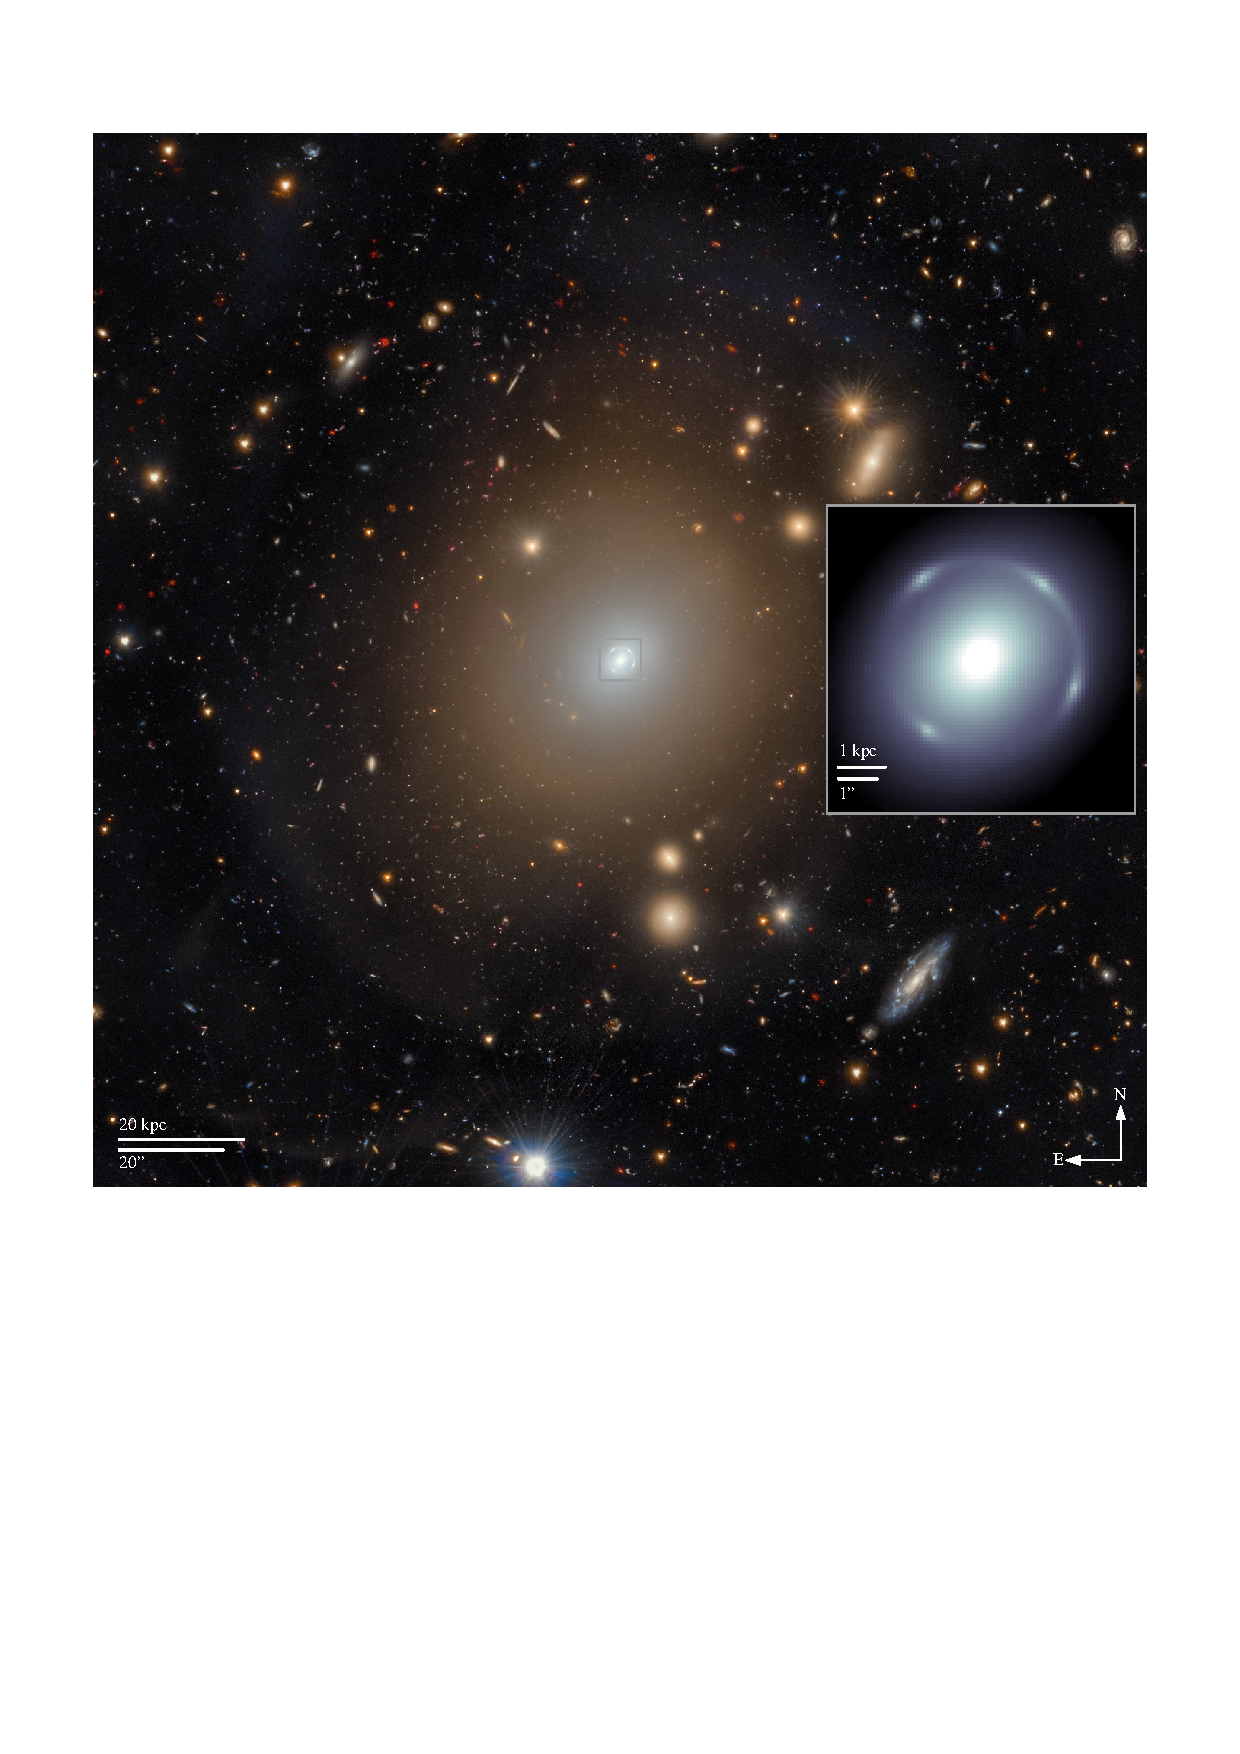
\includegraphics[width=1.0\linewidth]{aa53014-24-fig1.pdf}
        \caption{Euclid imaging of Altieri's lens, an example of an Einstein ring
        \cite{2025ORiordan}. The main panel shows a composite false-colour
        image constructed from Euclid VIS and NISP observations. The VIS instrument
        provides high-resolution optical imaging, while NISP provides lower-resolution
        near-infrared photometry in the $Y_E$, $J_E$, and $H_E$ bands. In this
        composite, the broadband VIS $I_E$ image defines the brightness structure,
        and the NISP bands provide the colour information. The central light of the
        lens galaxy has been suppressed to enhance the visibility of the lensed arc.
        The inset shows the central $8$ arcsec using only the higher-resolution VIS
        data, corresponding to the square marked in the main panel. The angular scale
        and the physical scale at the lens redshift are shown in each frame.}
        \label{fig:lensing}
    \end{figure}
\newpage    
\printbibliography %Prints bibliography
\end{document}
